\documentclass[times, utf8, seminar, numeric]{fer}

\usepackage{booktabs}
\usepackage{hyperref}
\usepackage{graphicx}
\usepackage{fancyhdr}
\usepackage{float}
\hypersetup{
	colorlinks=true,
	linkcolor=black,
	filecolor=magenta,      
	urlcolor=cyan,
	pdftitle={Overleaf Example},
	pdfpagemode=FullScreen,
}
\begin{document}


\title{Praćenje nogometaša primjenom YOLOv5 modela i DeepSORT algoritma}

\author{Marko Tutić}
\voditelj{Izv. prof. dr. sc. Zoran Kalafatić}
\maketitle

\tableofcontents

\chapter{Uvod}



Praćenje objekata je grana računalnog vida u kojoj se detekcije objekata u određenom okviru nastoje pratiti u nadolazećim okvirima.
Metode praćenja objekata se najčešće razvrstavaju u metode praćenja jednog objekta i metode praćenja više objekata. 
U metode praćenja jednog objekta ubrajaju se metode koje ne zahtijevaju detekciju objekta u svakom okviru videozapisa (engl. \textit{detection-free tracking}). U ovim metodama praćenja dovoljno je u početnom okviru zadati poziciju objekta koji se želi pratiti, a algoritam praćenja objekta zatim nastoji pratiti objekt u daljnjim okvirima na temelju karakteristika objekta i/ili promjena koje se događaju u slici.

Praćenje više objekata se realizira kao detektiranje objekata u nekom okviru i dodjeljivanje identifikatora dobivenim detekcijama. Cilj praćenja više objekata je očuvati identifikatore pojedinih objekata kroz više okvira videozapisa. Ovakva metoda praćenja objekata zahtjeva detekcije objekata u svakom okviru videozapisa (engl. \textit{tracking-by-detection}).
Praćenje više objekata često se vrši pod pretpostavkom da objekti neće naglo mijenjati brzinu i smjer kretanja.

Praćenje više objekata predstavlja veliki izazov u području računalnog vida jer se redovito javljaju situacije  poput zaklanjanja objekta ili mimoilaženja objekata u kojima može doći do pogrešnog ili propuštenog dodjeljivanja identifikatora objektima.
Zaklanjanje objekta je pojava kada objekt nije vidljiv na slici, ali je pozicija objekta i dalje sadržana unutar slike.
Mimoilaženje objekata može izazvati zamjenu identiteta te se ta pojava manifestira tako da se identifikator nekog praćenog objekta dodjeli drugom praćenom objektu, a identifikator drugog objekta dodjeljuje se početnom objektu. 


Praćenje nogometaša predstavlja situaciju u kojoj je potrebno pratiti više objekata pri čemu su moguće česte zamjene identiteta s obzirom na to da se igrači kroz trajanje cijele utakmice mimoilaze. Dodatan izazov pri praćenju nogometaša predstavlja činjenica da ako je kamera udaljena, igrači izgledaju vrlo slično zbog identičnih boja dresova te ih je stoga teže identificirati na temelju izgleda.

Za praćenje nogometaša na videozapisima izrađen je sustav za praćenje nogometaša koji se sastoji od djela za detekciju nogometaša i djela za praćenje na temelju detekcija. Dio sustava koji je zadužen za detekciju nogometaša koristi YOLOv5 model koji se uči na prikladnom skupu podataka, dok za se praćenje nogometaša koristi DeepSORT algoritam. DeepSORT algoritam koristi značajke koje opisuju izgled objekta te udaljenost detekcija i trajektorija kao kriterij dodjele detekcija trajektorijama.

Pozicije nogometaša u okvirima bilježe se za svakog nogometaša zasebno te se na temelju tih pozicija izrađuje mapa aktivnosti nogometaša. Pozicija nogometaša na terenu tretira se kao slučajna vektorska varijabla koja ima nepoznatu razdiobu pri čemu je mapa aktivnosti procjena funkcije gustoće te varijable. Funkcija gustoće se procjenjuje metodom procjene gustoće jezgre (engl. \textit{kernel density estimation}) pri čemu pozicije nogometaša dobivene analizom videozapisa predstavljaju uzorke pomoću kojih se vrši procjena.



\chapter{Skup podataka}

Za potrebe učenja i vrednovanja sustava za praćenje nogometaša  korišten je videozapis duljine 5 minuta koji sadrži snimku jedne nogometne utakmice te tekstualna datoteka koja sadrži oznake pozicija i identifikatora  nogometaša u svakom okviru tog videozapisa. Kamera kojom je utakmica snimana je statična. Svi okviri u videozapisu sadrže pregled cijelog nogometnog terena.
Jedna sekunda navedenog videozapisa sadrži 25 slikovnih okvira i širina okvira videozapisa iznosi 3260 piksela dok visina okvira iznosi 570 piksela.
Slika \ref{fig:okvir} prikazuje primjer jednog okvira videozapisa dok
slika \ref{fig:oznake} prikazuje primjer oznaka pozicija i identifikatora igrača u tekstualnoj datoteci za prvi okvir videozapisa.

\begin{figure}
	\centering
	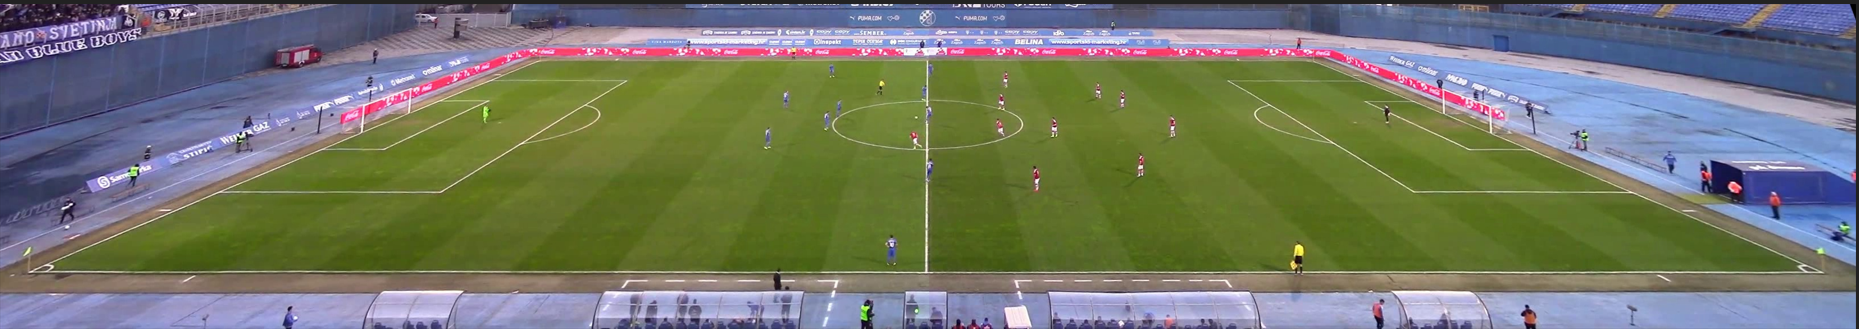
\includegraphics[width=\linewidth]{slike/okvir.png}
	\caption {Primjer okvira videozapisa}
	\label{fig:okvir}	
\end{figure}

Oznake pozicija igrača u okvirima videozapisa zapisane su u tekstualnoj datoteci u obliku propisanom MOT16 specifikacijom. Jedan redak tekstualne datoteke ima sljedeći format:

\textit{<redni broj okvira>, <identifikator igrača>, <x koordinata>, <y koordinata>, <širina>, <visina>, -1, -1, -1, -1.}


\begin{figure}
	\centering
	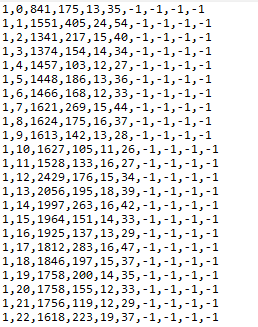
\includegraphics[scale=0.8]{slike/oznake.png}
	\caption {Primjer oznaka skupa podataka}
	\label{fig:oznake}	
\end{figure}



Koordinate \textit{x} i \textit{y} te širina i visina odnose se na pravokutnik koji omeđuje igrača na slici. Koordinate x i y označuju poziciju gornje lijeve točke tog pravokutnika. Na temelju gornje lijeve točke te širine i visine pravokutnika mogu se izvesti i ostale točke omeđujućeg pravokutnika čime je omeđujući pravokutnik u potpunosti definiran.
Niz brojeva -1 se ne koristi, no služe kao nadopuna za zadovoljavanje MOT16 formata.

Skup podataka dijeli se na skup za učenje, skup za provjeru i skup za testiranje. 
Okviri videozapisa se dijele u navedene skupove slijedno kako bi se očuvala mogućnost praćenja objekata u navedenim skupovima podataka. 

Skup podataka dijeli se tako da skup za učenje sadrži prvih 4500 okvira videozapisa, skup za provjeru sadrži idućih 1500 okvira, dok skup za testiranje sadrži preostalih 1515 okvira. 

Skup za učenje koristi se za učenje modela detekcije objekata. 
Skup za provjeru koristi se za provjeru svojstva generalizacije modela detekcije objekata tijekom različitih epoha učenja. 
Konačno, skup za testiranje koristi za vrednovanje modela detektora objekata nakon što je završen proces učenja. 

Za potrebe učenja detektora objekata oznake koje su zadane u MOT16 formatu potrebno je pretvoriti u oznake koje zadovoljavaju YOLOv5 format. YOLOv5 format specificira izradu tekstualne datoteke s oznakama za svaki okvir zasebno te se omeđujući pravokutnici u tim datotekama opisuju središtem omeđujućeg pravokutnika i njegovom širinom i visinom. Identifikatori igrača se ne uzimaju u obzir prilikom pretvorbe u YOLOv5 format jer je cilj detekcije objekata lokalizirati objekte i klasificirati ih. 

Dodatno je potrebno \textit{x} koordinatu i širinu omeđujućeg pravokutnika podijeliti sa širinom slike, odnosno \textit{y} koordinatu i visinu omeđujućeg pravokutnika potrebno je podijeliti s visinom slike. Takva pretvorba je potrebna jer model YOLOv5 na ulazu može primati slike različitih veličina te se pretvorbom postiže invarijantnost pozicije objekta na visinu i širinu slike. 


Iako se u DeepSORT algoritmu za praćenje objekata može naučiti konvolucijska neuronska mreža za izlučivanje značajki izgleda objekta pomoću istog skupa podataka, taj postupak je preskočen s obzirom na to da izvorni algoritam već sadrži naučenu mrežu za izlučivanje značajki osoba. Navedena mreža je prethodno naučena na MARS (Motion Analysis and Re-Identification Set) skupu podataka koji sadrži slike različitih osoba. 
Sustav za praćenje objekata vrednovat će se na skupovima za učenje i testiranje.




\chapter{Arhitektura sustava}

Sustav za praćenje nogometaša i generiranje mape aktivnosti sastoji se od 3 komponente:
\begin{itemize}
	\item Podsustav za detekciju pozicija nogometaša u okviru videozapisa
	\item Podsustav za praćenje nogometaša između okvira videozapisa
	\item Podsustav za generiranje mape aktivnosti na temelju rezultata dobivenih praćenjem nogometaša
\end{itemize}


\section{Detekcija nogometaša}
Za detekciju nogometaša na slici koristi se YOLOv5s model iz skupa modela YOLOv5. Karakteristike YOLOv5 modela je da sliku podijeli na ćelije te je svaka ćelija zadužena za detektiranje objekata kojima se središte nalazi u toj ćeliji. Sustav na ulazu prima slike koje predstavljaju okvire videozapisa te na izlazu vraća skup detekcija objekata na slici. Model vraća uvijek isti broj detekcija te je potrebno ukloniti redundantne detekcije primjenom algoritma potiskivanja nemaksimalnih odziva (engl. non-maximum suppression). S obzirom na to da se na terenu većinu vremena nalazi 22 nogometaša i jedan sudac, očekivani broj detekcija u svakom okviru iznosi 23. Model za detekciju objekata služi isključivo za određivanje pozicija nogometaša u trenutnom okviru, odnosno ne može identificirati pojedine objekte jer ne uzima u obzir detekcije iz prethodnih okvira. 	



\section{Praćenje objekata}
Za praćenje objekata koristi se algoritam DeepSORT.

Algoritam DeepSORT \cite{deepsort} nastao je kao proširenje SORT \cite{sort} algoritma koji se bazirao na korištenju Kalmanovog filtra za predviđanje trajektorija te mađarskog algoritma za dodjelu detekcija trajektorijama na temelju njihovog omjera presjeka i unije. Iako takav algoritam ima veliku brzinu izvođenja, navedeni algoritam karakterizira česta pojava zamjene identiteta. Za praćenje nogometaša, zamjena identiteta predstavlja veliki problem zbog česte interakcije među nogometašima te može rezultirati niskom preciznošću. Algoritam DeepSORT nastoji riješiti problem zamjene identiteta uvođenjem opisnika izgleda objekta koji se također uzima u obzir prilikom dodjele detekcija trajektorijama. Arhitektura neuronske mreže za dobivanje opisnika izgleda objekta prikazana je tablicom na Slici \ref{fig:deep_sort_net_arch}.
  
Algoritam također koristi Kalmanov filtar u svakoj trajektoriji za praćenje trenutnog stanja i predviđanje idućeg stanja, odnosno pozicije trajektorije u sljedećem okviru videozapisa. 
Predviđene trajektorije uspoređuju se s detekcijama na izlazu detektora objekata te se na temelju međusobne udaljenosti uparuju.
Udaljenost trajektorije i detekcije se definira kao težinska suma Mahalanobisove udaljenosti trajektorije i detekcije te kosinusne udaljenosti opisnika izgleda detekcije i trajektorije \cite{deepsort}. 

Uparivanje se vrši primjenom kaskadnog uparivanja koje se bazira na iterativnoj primjeni mađarskog algoritma pri čemu se prilikom uparivanja daje prioritet češće ažuriranim trajektorijama. Rezultat algoritma su uparene detekcije i trajektorije. Arhitektura sustava prikazana je na Slici \ref{fig:deep_sort_arch}.




\begin{figure}
	\centering
	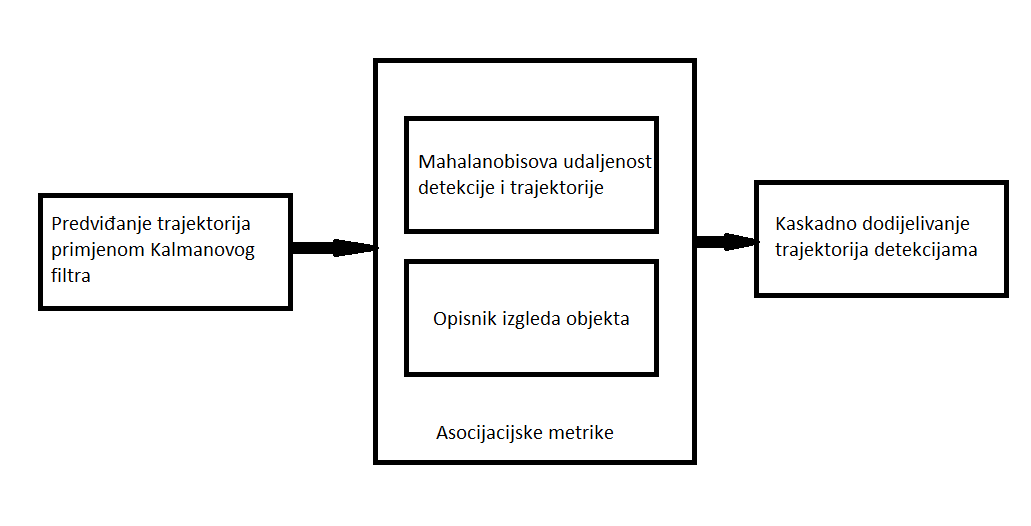
\includegraphics[width=\linewidth]{slike/deep_sort_arch.png}
	\caption {Arhitektura DeepSORT algoritma}
	\label{fig:deep_sort_arch}	
\end{figure}

\begin{figure}
	\centering
	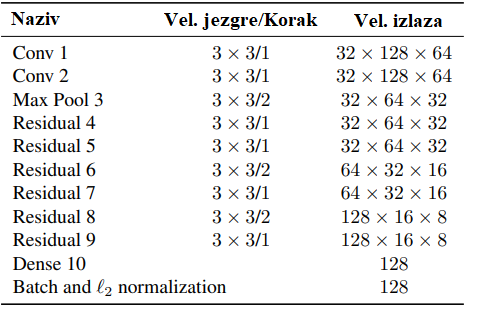
\includegraphics[scale=0.5]{slike/deep_sort_net_arch.png}
	\caption {Arhitektura opisnika izgleda}
	\label{fig:deep_sort_net_arch}
\end{figure}


\subsection{Kalmanov filtar}

Kalmanov filtar se u algoritmu DeepSORT koristi za praćenje internog stanja trajektorije te predviđanje pozicije objekta u nadolazećem okviru. Interno stanje trajektorije ažurira se kada je dostupan vektor mjerenja. Vektor mjerenja u kontekstu algoritma jednak je jednoj detekciji objekta. 

Algoritam DeepSORT stanje trajektorije definira kao 8-dimenzionalni vektor koji se sastoji od: \textit{x} koordinate objekta, \textit{y} koordinate središta objekta, omjera visine i širine, visine te brzina promjena za svaku od navedenih komponenti. Mjerenje se definira kao 4-dimenzionalni vektor koji se sastoji od: \textit{x} koordinate pozicije objekta, \textit{y} koordinate pozicije objekta, omjera visine i širine omeđujućeg pravokutnika objekta te visine tog pravokutnika. 


Za detekcije koje nisu uparene s postojećim trajektorijama prilikom procesa uparivanja, stvaraju se nove trajektorije koje su na početku u probnom stanju, odnosno još se ne tretiraju kao rezultat praćenja objekata. Tek ako se takvoj novostvorenoj trajektoriji dodjeli mjerenje kroz određen broj uzastopnih okvira, trajektorija prelazi u aktivno stanje te se tek tada tretira kao ispravna trajektorija. Tako se sprječava praćenje nepostojećih objekata koji bi nastajali kao posljedica lažno pozitivnih detekcija \cite{deepsort}.

Kada je trajektorija u aktivnom stanju te vektor mjerenja nije dostupan, odnosno detekcija nije dodijeljena, sljedeće stanje se predviđa pomoću internog stanja trajektorije \cite{sort}.
Ako se nekoj aktivnoj trajektoriji ne dodjeli mjerenje unutar određenog broja uzastopnih okvira, trajektorija i njeno stanje se briše. \cite{deepsort}.
Trajektorija kojoj nije dodijeljeno mjerenje se ne prikazuje na izlazu sustava sve dok se trajektoriji ponovo ne dodijeli neka detekcija.

\subsection{Dodjela trajektorija detekcijama}

U svakom okviru potrebno je dodijeliti detekcije trajektorijama tako da parovi detekcija i trajektorija budu minimalno udaljeni.
Algoritam DeepSORT ne pokušava upariti sve detekcije i trajektorije odjednom već daje prednost trajektorijama kojima se interno stanje češće ažurira pomoću novih mjerenja, odnosno detekcija. 
Algoritam kreće od dodjeljivanja nedodijeljenih detekcija najčešće ažuriranim trajektorijama. 

Kriterij koji se razmatra prilikom uparivanja trajektorija i detekcija sastoji se od dvije komponente: kvadrirane Mahalanobisove udaljenost između predviđene pozicije objekta (dobiva se primjenom Kalmanovog filtra) i detekcije te minimalne kosinusne udaljenosti između opisnika izgleda detektiranog objekta i prethodnih opisnika objekta za određenu trajektoriju. Za jednu trajektoriju se pamti određen broj opisnika izgleda detekcija koje su bile prethodno uparene s tom trajektorijom. Navedene udaljenosti se linearno kombiniraju u konačnu udaljenost koja se razmatra prilikom dodjele detekcija trajektorijama.

Trajektorije i detekcije s minimalnom udaljenošću uparuju se uzimajući u obzir ažurnost trajektorija i prag udaljenosti koji ni jedna dodjela ne smije prekoračiti. Rezultat uparivanja s ovim ograničenjima je da će neke trajektorije biti uparene s nekim detekcijama, ali i dalje mogu ostati neuparene detekcije i neuparene trajektorije. U idućem koraku ponovo se uzimaju  neuparene trajektorije koje su rjeđe ažurirane od prethodno uparenih te se pokušavaju upariti s preostalim neuparenim detekcijama. 

Kao parametar algoritma se postavlja maksimalni broj okvira, odnosno maksimalno vrijeme koje je prošlo od ažuriranja trajektorije te se ono koristi za određivanje koliko puta će pokušati dodijeliti neuparene detekcije neuparenim trajektorijama. 

Ako nakon ovakvog iterativnog dodjeljivanja i dalje postoje neuparene detekcije i trajektorije, one se uparuju primjenom mađarskog algoritma gdje se kao kriterij optimizacije prilikom dodjeljivanja koristi omjer presjeka i unije između područja detekcije i predviđenog područja trajektorije. Za ovo dodjeljivanje se također uvodi prag koji mora biti zadovoljen kako bi se uparivanje smatralo uspješnim\cite{deepsort}.

Ako i dalje postoje neuparene detekcije, za njih se stvaraju nove trajektorije koje zatim moraju proći probnu fazu. Neuparene trajektorije ne dobivaju mjerenje u tom okviru te ako su u aktivnom stanju, same predviđaju svoju poziciju primjenom Kalmanovog filtra.


\section{Izrada mape aktivnosti}

Mape aktivnosti izrađuju se nakon analize cijelog videozapisa. Mape aktivnosti se izrađuju za svakog nogometaša zasebno te se pohranjuju kao slike. 
Za izradu mape aktivnosti, koristi se slika igrališta iz ptičje perspektive kao pozadina. Navedena slika prikazana je na Slici \ref{fig:pitch}. 

\begin{figure}
	\centering
	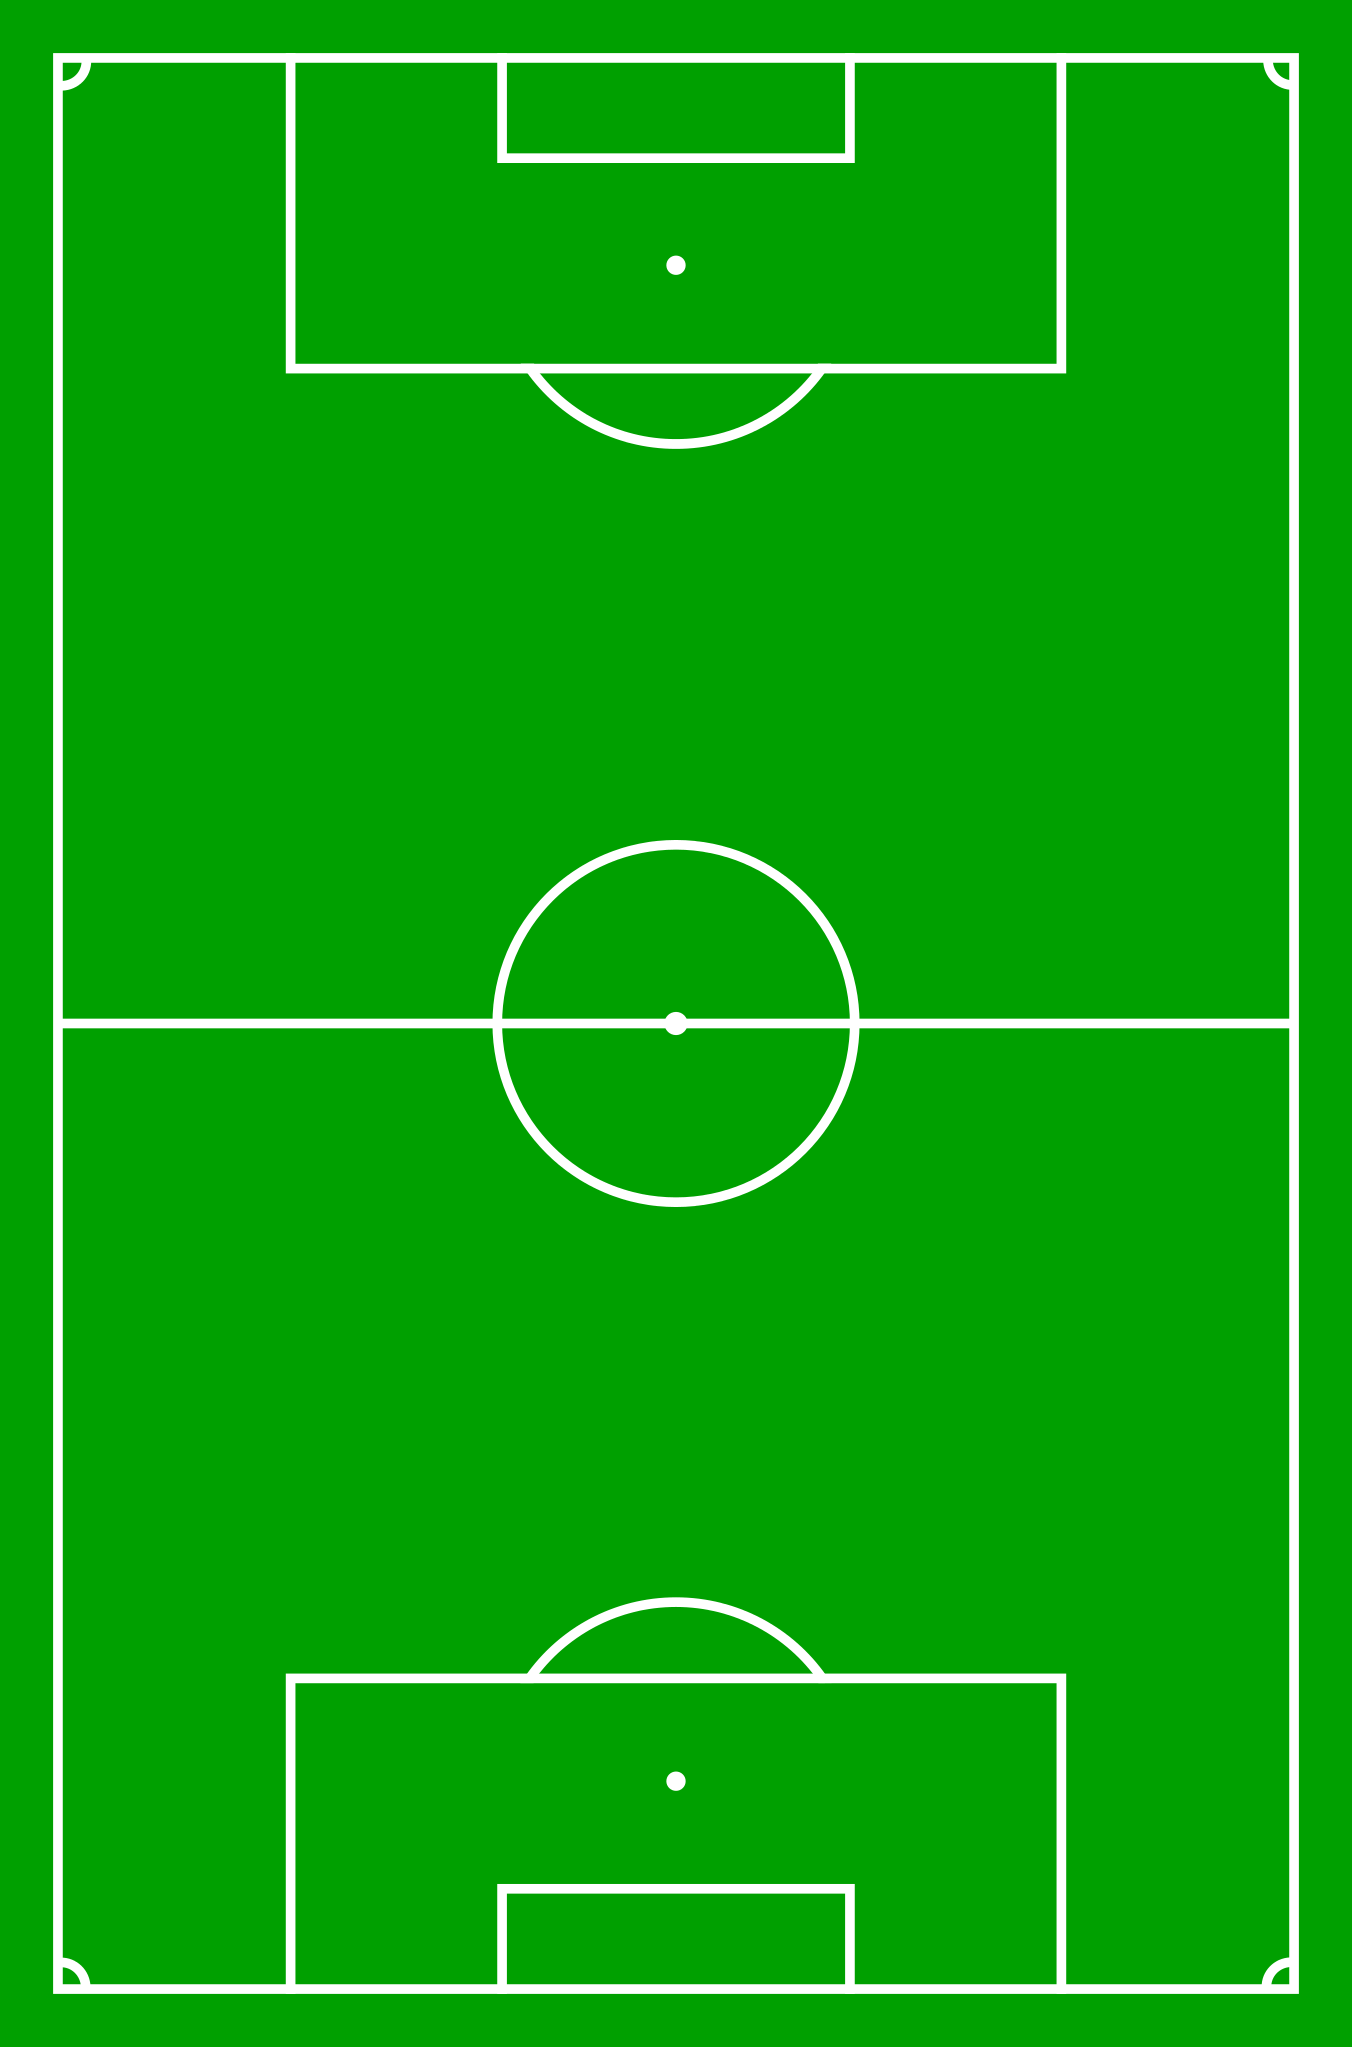
\includegraphics[scale=0.15]{slike/pitch.png}
	\caption {Nogometni teren iz ptičje perspektive}
	\label{fig:pitch}	
\end{figure}

Na početku se za svakog igrača izrađuju liste x i y koordinata njihovih pozicija na okvirima videozapisa. 
Za poziciju igrača odabrana je točka koja se nalazi na polovištu donje lijeve i donje desne točke omeđujućeg pravokutnika detekcije igrača.

Pozicije igrača na okvirima videozapisa ne moraju odgovarati pozicijama na slici terena iz ptičje perspektive te je stoga potrebno provesti perspektivnu transformaciju.  
Za dobivanje matrice perspektivne transformacije potrebno je zadati četiri točke koje predstavljaju pozicije rubova igrališta u videozapisu te četiri točke koje predstavljaju rubove igrališta na slici terena iz ptičje perspektive. 

Na temelju tih točaka izračunava se transformacijska matrica pomoću koje se sve točke koje predstavljaju pozicije igrača u okviru videozapisa preslikavaju u poziciju igrača na terenu snimljenom iz ptičje perspektive. S obzirom na to da se pozicija kamere može razlikovati u pojedinim videozapisima, potrebno je za svaki videozapis precizno zadati točke koje predstavljaju rubove terena, jer će u protivnom rezultirajuće mape aktivnosti biti netočne.

Jednom kada su sve točke pozicija u okvirima preslikane u odgovarajuće točke pozicija na terenu iz ptičje perspektive, izračunava se mapa aktivnosti. Pozicije nogometaša tretiraju se kao slučajne varijable koje imaju nepoznatu funkciju gustoće. Za procjenu te razdiobe koristi se metoda procjena gustoće jezgre. Konačan rezultat je procijenjena funkcija gustoće pozicija koja ujedno predstavlja i mapu aktivnosti nekog igrača. Primjer jedne mape aktivnosti prikazan je na Slici \ref{fig:heatmap}

\begin{figure}
	\centering
	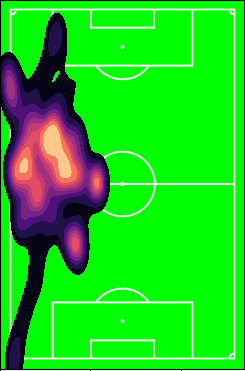
\includegraphics[scale=1]{slike/heatmap.png}
	\caption {Mapa aktivnosti za igrača}
	\label{fig:heatmap}	
\end{figure}


\chapter{Implementacija sustava}

\section{Podsustav za detekciju nogometaša}


Podsustav za detekciju nogometaša sastoji se YOLOv5 detektora objekata koji na ulazu prima slikovne okvire videozapisa, a na izlazu vraća detekcije s podacima o detekciji. 
Implementacija YOLOv5 detektora preuzeta je s izvornog repozitorija \cite{yolov5impl}. Iz repozitorija je iskorištena skripta za učenje modela detekcije i skripta za vrednovanje naučenog modela. 

Prilikom implementacije sustava praćenja nogometaša iz repozitorija se dodatno iskorištavaju sljedeće funkcije:
\begin{itemize}
	\item funkcija za izvođenje unaprijednog prolaza za određenu sliku
	\item funkcija za primjenu potiskivanja nemaksimalnih odziva s ciljem uklanjanja redundantnih i višestrukih detekcija
	\item funkcija za dohvaćanje naučenog modela
	\item funkcije za iscrtavanje izlaznih detekcija na okvirima izlaznog videozapisa 
\end{itemize}


Za potrebe prilagodbe skupa podataka YOLOv5 formatu izrađena je skripta \textit{dataset\textunderscore builder.py}. Navedena skripta slijedno čita okvire videozapisa i za svaki okvir stvara sliku i prikladnu tekstualnu datoteku s oznakama u YOLOv5 formatu. 
Dodatno je izrađena skripta \textit{dataset\textunderscore splitter.py} koja slike i oznake dobivene skriptom \textit{dataset\textunderscore builder.py} dijeli u skup za učenje, skup za provjeru i skup za testiranje.

\section{Podsustav za praćenje nogometaša}

Za praćenje nogometaša koristi se algoritam DeepSORT. 
Implementacija navedenog algoritma također je preuzeta s izvornog repozitorija \cite{Wojke2018deep}\cite{deepsort}. 
Algoritam DeepSORT koristi detekcije objekata i značajke izgleda prilikom izračuna udaljenosti detekcija i trajektorija. Detekcije objekata se dobivaju iz modela YOLOv5s, dok se značajke izgleda objekata dobivaju iz neuronske mreže za izlučivanje značajki.

Za izlučivanje značajki može se koristiti bilo koji model neuronske mreže koji na izlazu daje vektor značajki, odnosno model neuronske mreže koji ima ulogu enkodera. Učenje neuronske mreže za izlučivanje značajki u implementaciji sustava nije napravljeno, već je iskorišten izvorni model koji je naučen izlučivati značajke osoba.

U implementaciji sustava korišteni su sljedeći parametri algoritma DeepSORT: 
\begin{itemize}
	\item potrebne su 3 uzastopne detekcije dodijeljene trajektoriji prije nego što trajektorija postane aktivna
	\item najveća dozvoljena kosinusna udaljenost prilikom dodijele detekcija trajektorijama iznosi 0.3
	\item trajektorija se briše ako se ne upari ni s jednom detekcijom u uzastopnih 100 okvira
	\item jedna trajektorija sprema posljednjih 200 vektora značajki izgleda objekata s kojima uspoređuje vektore značajki detekcija prilikom dodjeljivanja detekcija trajektorijama
	\item najmanji dozvoljeni omjer presjeka i unije između detekcije i trajektorije prilikom dodjele iznosi 0.1
\end{itemize}

Navedene vrijednosti parametara određene su eksperimentalno na skupu podataka za učenje.


\section{Podsustav za izradu mape aktivnosti nogometaša}

Dio sustava zadužen za generiranje mapi aktivnosti implementiran je pomoću skripte \textit{heatmap\textunderscore builder.py}.
Skripta za izradu mape aktivnosti pojedinih nogometaša koristi tekstualnu datoteku s pozicijama nogometaša u MOT16 formatu iz koje se za svakog nogometaša stvara lista njegovih pozicija u videozapisu. 
Pozicija nogometaša se tretira kao slučajna varijabla, odnosno mapa aktivnosti predstavlja funkciju gustoće distribucije pozicije igrača. 
Navedena funkcija gustoće aproksimira se pomoću metode procjene gustoće jezgre pri čemu pozicije nogometaša predstavljaju uzorke funkcije gustoće koja se procjenjuje. 
Procjena funkcije gustoće definirana je formulom:

\[\hat{f_h}(\vec{x}) = \frac{1}{nh} \sum_{i=1}^{n} K( \frac{\vec{x} - \vec{x_i}}{h}) \]

% TODO citiraj wikipediu
Za aproksimaciju funkcije i njen slikovni prikaz koristi se funkcija \textit{kdeplot} iz knjižnice \textit{Seaborn}. Slika \ref{fig:pitch} koja prikazuje nogometni teren iskorištena je kao pozadina mape aktivnosti. 
Rezultat izvođenja skripte \textit{heatmap\textunderscore builder.py} su slike mapa aktivnosti svih detektiranih igrača.

\section{Povezivanje podsustava u cjelinu}

Glavna skripta \textit{system.py} na početku inicijalizira podsustav za praćenje objekata. Za inicijalizaciju podsustava potrebno je navesti putanju do datoteke s informacijama o modelu za izlučivanje značajki te je potrebno navesti parametre algoritma DeepSort navedene u potpoglavlju 4.2.

Nakon inicijalizacije sustava za praćenje, inicijalizira se sustav za detekciju objekata. Za inicijalizaciju navedenog sustava potrebno je navesti putanju do datoteke koja sadrži informacije o naučenom modelu te sklopovlje na kojem će se izvršavati detekcija nogometaša.

Sustav na izlazu daje videozapis s označenim nogometašima te je stoga potrebno stvoriti razrede za izradu videozapisa te se oni stvaraju nakon inicijalizacije sustava za detekciju objekata.

Nakon inicijalizacije podsustava za detekciju i praćenje, iterativno se obrađuju okviri videozapisa tako da se za svaki okvir provodi detekcija objekata, potiskivanje nemaksimalnih odziva, dodjeljivanje detekcija trajektorijama te na kraju izrada i dodavanje okvira s rezultatima na kraj izlaznog videozapisa.

\section{Podsustav za vrednovanje praćenja i detekcije objekata}

Za evaluaciju detekcije objekata korištena je skripta \textit{val.py} iz implementacije YOLOv5 detektora. Navedena skripta na ulazu prima model i skup podataka nad kojima vrši vrednovanje. Skripta na temelju ulaza generira podatke koji opisuju kvalitetu modela detekcije poput preciznosti, odziva, F1-mjere i mnogih drugih.

% TODO citiraj mot evaluator
Za evaluaciju praćenja objekata iskorišten je program TrackEval koji kao ulaz zahtjeva datoteku s pozicijama pojedinih objekata koje je dao sustav i datoteku sa stvarnim pozicijama objekata. Program zahtjeva da obje datoteke sadrže pozicije i identitete objekata u MOT16 formatu.
Rezultat programa je ispis raznih mjera koje ocjenjuju performanse algoritma za praćenje objekata.


\chapter{Analiza rezultata}
\section{Vrednovanje modela detekcije nogometaša}

Model detekcije nogometaša vrednovat će se na skupu za učenje te na skupu za testiranje. Za svaki skup mjerit će se preciznost, odziv, F1-mjera, sredina prosječnih preciznosti kada je prag omjera presjeka i unije 0.5 te sredina prosječnih preciznosti za pragove omjera presjeka i unije u rasponu od 0.5 do 0.95.

Preciznost za binarnu klasifikaciju se definira kao omjer stvarno pozitivnih detekcija i zbroja stvarno pozitivnih detekcija i lažno pozitivnih detekcija. Preciznost modela detekcije nogometaša iznosi na skupu za učenje iznosi 0.907, dok na skupu za testiranje preciznost iznosi  0.878.

Odziv se definira kao omjer stvarno pozitivnih detekcija i zbroja stvarno pozitivnih detekcija i lažno negativnih detekcija te ona za naučeni model na skupu za učenje iznosi 0.89, dok na skupu za testiranje iznosi 0.816.

F1-mjera definira se kao harmonijska sredina preciznosti i odziva te ona iznosi 0.892 na skupu za učenje, odnosno 0.846 na skupu za testiranje.
Na slikama 4.1 i 4.2  prikazana je krivulja preciznosti u ovisnosti o odzivu (engl. \textit{precision-recall curve}).


Sredina prosječnih preciznosti za prag omjera presjeka i unije 0.5 (\(mAP@0.5\)) definira se kao aritmetička sredina prosječnih preciznosti (\(AP_i@0.5\)) za svaki razred \(i\) pri čemu prosječne preciznosti također koriste prag omjera presjeka i unije iznosa 0.5 prilikom određivanja točnih detekcija.
Prag omjera presjeka i unije definira kada se neka detekcija smatra ispravnom. Za konkretni slučaj kada je omjer presjeka i unije detekcije objekta i stvarne pozicije objekta veći od 0.5, detekcija se smatra ispravnom.	
Prosječna preciznost definira se kao površina ispod krivulje preciznosti u ovisnosti o odzivu.
Sredina prosječnih preciznosti na skupu za učenje iznosi 0.907, dok na skupu za testiranje iznosi 0.84. 

Sredina prosječnih preciznosti za pragove omjera presjeka i unije u rasponu od 0.5 do 0.95 definira se kao prosjek sredina prosječnih preciznosti za sljedeće pragove omjera presjeka i unije: 0.5, 0.55, 0.6, 0.65, 0.7, 0.75, 0.8, 0.85, 0.9, 0.95.
Navedena mjera na skupu za učenje iznosi 0.467, dok na skupu za testiranje iznosi 0.37.

Visoka preciznost, odziv i F1-mjera ukazuju na dobra svojstva generalizacije naučenog modela. 
Mala vrijednost sredine prosječnih preciznosti za pragove omjera presjeka i unije u rasponu od 0.5 do 0.95 ukazuje na manje preciznu lokalizaciju pri visokim pragovima omjera presjeka i unije, odnosno kada je prag omjera presjeka i unije vrlo visok, detektor daje manje ispravnih detekcija.
Vrijedi napomenuti kako je sustav naučen detektirati nogometaše samo na jednom videozapisu, odnosno snimci jedne utakmice. Vrednovanje ovakvog modela detekcije na nekoj drugoj snimci mogao bi rezultirati manjom preciznošću. Za ostvarenje mogućnosti šireg korištenja modela, potrebno je naučiti model na više snimki nogometnih utakmica te bi bilo poželjno da su uvjeti u kojima se igraju utakmice različiti.

\section{Vrednovanje algoritma praćenja objekata}

Za vrednovanje praćenja objekata koristit će se sljedeće metrike:

\begin{itemize}
	\item točnost praćenja više objekata (engl. \textit{multiple object tracking accuracy}, MOTA)
	\item preciznost praćenja više objekata (engl. \textit{multiple object tracking precision}, MOTP)
	\item broj većinom praćenih objekata (engl. \textit{mostly tracked}, MT)
	\item broj djelomično praćenih objekata (engl. \textit{partially tracked}, PT)
	\item broj većinom izgubljenih objekata (engl. \textit{mostly lost}, ML)
	\item broj zamjena identiteta (IDSW)
	\item broj fragmentacija (FM)	
\end{itemize}

Točnost praćenja više objekata definira se formulom:

\[MOTA = 1- \frac{\sum_{t}(FN_t + FP_t + IDSW_t)}{\sum_{t} GT_t}\]

pri čemu se u brojniku za svaki okvir zbrajaju broj lažno pozitivnih i lažno negativnih objekata te broj zamjena identiteta. U nazivniku se u svakom okviru zbraja broj objekata koji je u tom okviru sadržan. Točnost praćenja na skupu za učenje iznosi , a na testnom skupu iznosi 60.00\%.



Preciznost praćenja više objekata definira se formulom:

\[MOTP = \frac{\sum_{t,i} d_{t,i}}{\sum_{t} c_t}\]

gdje \(d_{t,i}\) predstavlja preklapanje omeđujućeg pravokutnika \(i\)-te trajektorije i stvarne vrijednosti, dok \(c_t\) predstavlja broj uspješnih dodjeljivanja u okviru \(t\). Preciznost praćenja nogometaša na skupu za učenje iznosi, dok na testnom skupu iznosi 33.33\%.


Većinom praćen objekt je onaj objekt kojeg algoritam za praćenje objekata uspješno prati u više od 80\% okvira. Broj većinom praćenih objekata u sustavu iznosi 1.

Djelomično praćen objekt je objekt kojeg algoritam za praćenje prati u rasponu od 20\% do 80\% okvira te broj takvih objekata u izrađenom sustavu za praćenje nogometaša iznosi 22.

Većinom izgubljeni objekti su oni objekti koje algoritam za praćenje uspijeva pratiti u manje od 20\% okvira. Sustav za praćenje nogometaša na skupu za testiranje kao ni na skupu za učenje nema takvih objekata.

Broj zamjena identiteta je značajan unatoč korištenju opisnika izgleda objekata te iznosi 66 za testni skup.

Prilikom praćenja objekata zbog mimoilaženja nogometaša na slici, često dolazi do zaklanjanja koje rezultira fragmentacijom. Fragmentacija mjeri broj situacija u kojima se objekt prestaje pratiti te se nakon određenog broja okvira ponovo nastavi pratiti. Broj fragmentacija na skupu za učenje iznosi , a na testnom skupu iznosi 2538.


\chapter{Zaključak}

Praćenje nogometaša zahtjevan je zadatak zbog čestih promjena u kretanjima nogometaša. Veliki broj algoritama praćenja objekata pretpostavlja linearan model kretanja objekata u kojem se između okvira ne događaju velike promjene u brzini kretanja objekata što u slučaju kretanja nogometaša ne mora vrijediti. Praćenje dodatno otežavaju česte interakcije nogometaša koje vrlo lako mogu izazvati zamjenu identiteta i zaklanjanje pojedinih nogometaša. 

Za praćenje nogometaša izrađen je sustav koji se bazira na detekciji svih nogometaša primjenom YOLOv5 modela te na dodjeli identiteta dobivenim detekcijama primjenom DeepSORT algoritma. 

Model za detekciju objekata YOLOv5s pokazuje dobra generalizacijska svojstva na korištenom skupu podataka, unatoč tome što je za detekciju bio korišten najmanje složen model iz skupa modela koje sadrži YOLOv5. S obzirom na to da igrači na snimci zauzimaju relativno mali udio okvira u odnosu na pozadinu, potreban je detektor koji radi sa slikama visoke rezolucije te je stoga naučeni model za detekciju koristio ulazne slike širine 1504. U protivnom se događa veliki gubitak informacije i dolazi do značajnog pada preciznosti detektora. 

Algoritam za praćenje DeepSORT unatoč korištenju opisnika izgleda objekta i dalje rezultira relativno čestim zamjenama identiteta objekata prilikom interakcija između nogometaša. Kada nema navedenih interakcija, algoritam daje zadovoljavajuće rezultate, odnosno prati objekte s visokom preciznošću. Preciznost algoritma praćenja ovisi i o korištenom modelu detekcije objekata jer algoritam DeepSORT ažurira trajektorije pomoću detekcija objekata u svakom okviru videozapisa te je stoga poželjno imati detektor objekata vrlo visoke preciznosti. 

Generiranje mape aktivnosti uvelike se oslanja na pozicije objekata dobivene praćenjem objekata te su poželjna što duža praćenja nogometaša u snimci, u protivnom se pojedina područja aktivnosti nogometaša ne bilježe i mapa aktivnosti poprima drugačiji oblik od očekivanog. Također na izgled mape aktivnosti utječu i zamjena identiteta te privremena zaklanjanja nogometaša.


\bibliography{literatura}
\bibliographystyle{fer}

\end{document}
